\documentclass[a4paper,12pt]{article}
\usepackage[utf8]{inputenc}
\usepackage{graphicx}
\usepackage{graphics}
\usepackage{hyperref}
\usepackage{geometry}
\usepackage{comment}
\graphicspath{ {build/} } 
\geometry{left=2cm, right=2cm, top=2cm, bottom=2cm}

\begin{document}

\begin{titlepage}
    \begin{center}
        \vspace*{3cm}
        
        {\Huge \textbf{Laboratorio 1 - Grupo 7}}\\[1cm]
        {\LARGE Panel solar automático:\\ [0.5cm]Planificación y Gestión de Proyecto}\\[2cm]
        
        \vfill
        
        {\Large \textbf{Integrantes }}\\[.5cm]
        \large
        \begin{tabular}{c c}
            Gartner, Francisco Nehuen & 69864/6 \\
            Marchesotti, Guido Daniel & 69923/9 \\
            Rosa, Fausto Pablo & 69843/1 \\
        \end{tabular}
        
        \vspace{1cm}
        
        \begin{figure}[b]
            \centering
            
\includegraphics[width=1\linewidth]{LOGOSFI-UNLP-color-01.png}
        \end{figure}
        
        %%{\large \today}
    \end{center}
\end{titlepage}

%%\newpage
%%\tableofcontents
%%\newpage

\section{Acta de constitución de Proyecto}

\hspace{0.4cm}\textbf{ Visión general del proyecto}: 
Desarrollar un sistema de seguimiento solar que optimice la captación de energía, controlando la orientación del panel solar según la posición del sol y transmitiendo la información generada a través de una interfaz gráfica.

\textbf{Objetivos}: 
\begin{itemize}
    \item \textbf{General}: sistema de control de panel solar. Se propone como proyecto la creación de un sistema que rote siguiendo la trayectoria del sol, con el fin de obtener la mayor potencia instantánea posible. Este sistema busca mejorar la eficiencia en comparación con los paneles solares estáticos. Las medidas de potencia, y su horario de medición, van a ser almacenadas y transmitidas para luego ser visualizadas en una interfaz gráfica que incluirá gráficos adicionales y datos históricos de la eficiencia del panel.
    \item \textbf{Particular}: se desarrollarán los siguientes apartados:
    \begin{itemize}
        \item Sistema de rotación
        \item Manejo de energía del micro
        \item Circuito de medición de potencia
        \item Desarrollo de comunicación entre dispositivos
        \item Creación de interfaz gráfica para móvil
        \item Programación de sistema de control
        \item Alimentación del sistema
        
    \end{itemize}

    
\end{itemize}

\textbf{Especificaciones y Alcance}:
\begin{itemize}
    \item \textbf{Requisito funcional}: El sistema debe ser capaz de ajustar su posición adaptándose a los cambios de incidencia solar para obtener la máxima potencia posible. Deberá ser capaz de medir correctamente la potencia para luego transmitir esos datos vía Bluetooth a una interfaz gráfica accesible desde una aplicación de celular. El sistema debe ser eficiente energeticamente en comparación con un típico panel solar estático, donde la potencia adicional obtenida con este proyecto sea apreciable.Además, se espera que el sistema sea autosustentable, pudiendo generar mas energía que la que se consumirá en su totalidad.
    \item \textbf{No funcional}: El sistema debe ser robusto y capaz de operar durante largos periodos de tiempo sin fallas. La interfaz gráfica debe ser intuitiva para operarios. Debe sentar una base confiable para proyectos futuros de mayores dimensiones o escalado del proyecto.
    \item \textbf{Alcance}: Principalmente, el proyecto abarcará desde el diseño y fabricación del hardware hasta el desarrollo de software. De objetivo secundario, deberá contar con una batería que se cargue con el remanente de energía. No se incluye producción en masa, solo un prototipo funcional y operativo.
\end{itemize}

\textbf{Entregables}: 
Prototipo final ensamblado, código fuente del microcontrolador, interfaz gráfica, breve documentación de uso, resultados de pruebas obtenidos y bitácora de desarrollo. \newline

\textbf{Presupuesto estimado :} Considerando los precios de los controladores, sensores comerciales, precios regionales y un margen flexible se propone el siguiente presupuesto de   \$100.000

\begin{comment}
\newpage
\section{Planificación y Gestión de Proyecto}

\begin{itemize}
    \item \textbf{Ciclo de vida}: ciclo de vida híbrido. Semi-flexible. Implementación clara y particular. Los alcances del proyecto son especificados al inicio del mismo. No se espera hacer grandes ajustes, pero se espera adaptabilidad a los plazos.
    \item \textbf{Organización del equipo de trabajo}: implementación de tareas rotativas.
    \item \textbf{Desglose de actividades}:
    \begin{itemize}
        \item Primera etapa de planificación: propósito, materiales, costos, cronograma, recopilación de información, división de tareas.
        \item Segunda etapa de planificación: realización de planos y esquemas.
        \item Obtención de insumos.
        \item Desarrollo de software de etapa temprana.
        \item Realización de maquetas y prototipos.
        \item Acondicionamiento y etapa de pruebas.
        \item Etapa alfa.
        \item Puesta a punto y modificaciones finales.
        \item Entrega del proyecto final.
    \end{itemize}

    \begin{figure}[h!]
        \makebox[0pt]{%
        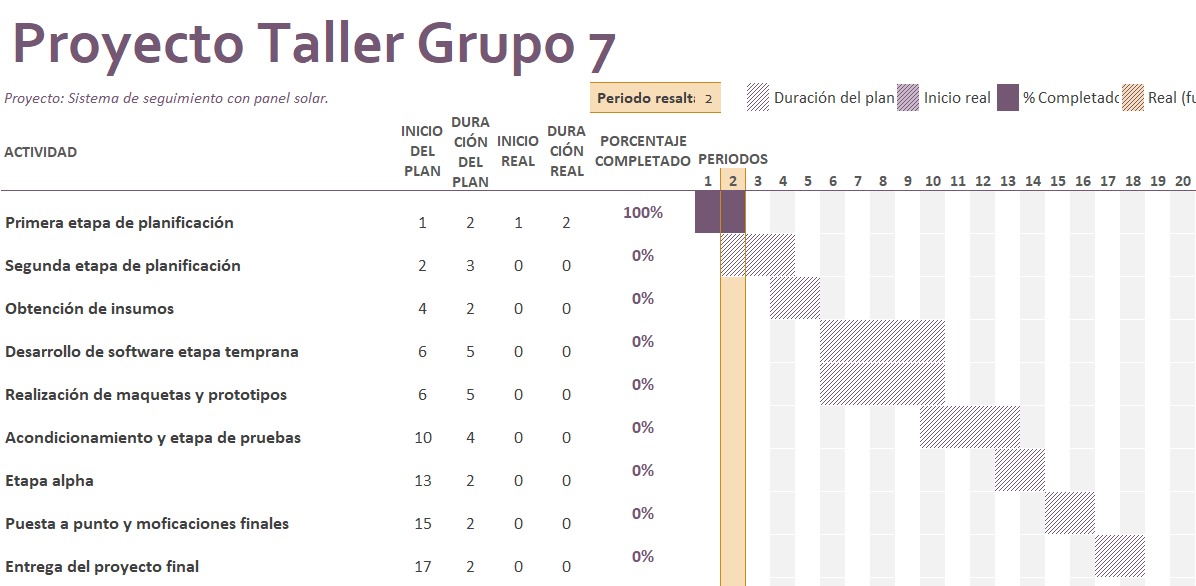
\includegraphics[width=0.9\paperwidth]{Gantt_2semana}}
        \centering
        \caption{Info \label{overflow}}
    \end{figure}

    \item \textbf{Adquisiciones}: 
    \begin{itemize}
        \item Sensores
        \item Panel solar
        \item Motores
        \item Soporte 
        \item Microcontrolador
        \item Transmisor de datos
        \item Sistema de Alimentación 
    \end{itemize}

    \item 
    \textbf{Costos estimados :} En base al anterior listado se propone un presupuesto de   \$100.000
\end{itemize}
\end{comment}
\end{document}
